\subsection{Sensitivity}\label{sec:eval:sens}

Figure~\ref{fig:sens} varies the two decision parameters of the return and the visibility the scan planner faces. The
return sweeps run the coupled policy on three cities (Shenzhen, New York, SynthCity), clear weather and rain, three
seeds and all 25 combinations of the two margins; every combination flies the same sorties.

\paragraph{Clearance margin.} The margin above the corridor top trades launches for headroom
(Fig.~\ref{fig:sens}a). No setting from 0 to 20\,m lets a drone touch a building, because the clearance envelope
already contains a 10\,m safety margin and a 4\,m dilation. Larger margins raise the cruise and return altitudes,
which costs energy: at 20\,m the precheck declines 38.2\% of sorties instead of 27.1\% at the default of 5\,m, and
completion falls from 59.0\% to 50.7\%. Below 5\,m the gain is at most 1.4 points. The only contact in the sweep at a
margin of 0\,m is between two drones whose transit and return paths then coincide; inter-drone separation is handled by
the runtime's separation guard, not by the return planner.

\paragraph{Trigger margin.} The return starts when the remaining flight time falls below a multiple of the
energy-equivalent return time. Between 1.0 and 1.5 the outcome does not change (Fig.~\ref{fig:sens}b): with the shared
energy model the trigger is rarely the binding constraint, because the precheck has already budgeted the return. At 1.8
it recalls 16.7\% of sorties early instead of 13.9\% and completes 4.2 points fewer. The default of 1.3 sits in the flat
region, so the result does not depend on tuning it.

\paragraph{Visibility.} The coupled scan planner keeps capture within a few points of the clear-air ceiling down to a
MOR of about 200\,m (Fig.~\ref{fig:sens}c), where the weather-blind plan has already lost almost every target
(Fig.~\ref{fig:m3}a). It pays with drones: a recognition scan needs 1.76 drones on average in clear air, 2.29 at
200\,m and 3.19 at 100\,m. At 100\,m capture drops to 51--74\%, and 19--43\% of the plans are declined because no
lens resolves the target from a height that clears the buildings; the planner reports this before launch. The wind
sweep of Fig.~\ref{fig:m2} gives the corresponding sensitivity of launch and return to wind speed.

\begin{figure}[t]
\centering
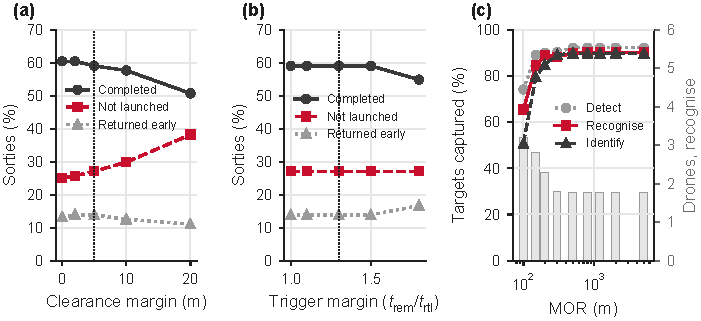
\includegraphics[width=\textwidth]{figures/pdf/sensitivity.pdf}
\caption{Sensitivity of the coupled policy. (a) Clearance margin above the corridor top and (b) return-trigger margin,
on the same 216 sorties per setting in clear weather and rain; dotted lines mark the defaults. (c) Scan planning under
a MOR sweep: targets captured at each level (lines, left axis) and drones a recognition scan needs (bars, right axis)}
\label{fig:sens}
\end{figure}
